\section{Fractal}

\emph{フラクタル}は数学者ブノワ・マンデルブロが提唱した幾何学の概念である.
自己相似性をもつ図形はどこを拡大しても全体と同じ形を見ることができる.
図\ref{fig:gasket}は\emph{シェルピンスキーのギャスケット}と呼ばれるフラクタル図形である.
三角形を一定の法則に基づいて分割していくことで,無限に続いていく三角形が得られる.
その形はどこを拡大しても同様の法則性を持った図形が得られる.
また,自然界の多くの場面でもフラクタル構造をみることができる. 
海岸線や, シダ植物などにもフラクタル構造をみることができる. 
フラクタルを考えることは自然科学研究の新たなアプローチとしても発展した. 

自己相似性を持つ図形はフラクタルという名がつけられる以前から研究されていた.
また,アートとしてもフラクタルを連想するような作品が存在していたが,
コンピュータが普及することによって,様々なフラクタル図形を描画することができるようになり,アートとしても大きく発展した.
この章ではコンピュータで計算,描画されるフラクタルを紹介する.

アートやコンピュータ文化との関連は切り離せない. これらのフラクタルは多くの場合数学的な研究対象にならないものの.
Fractal Forum\footnote{Fractal Forum:  \url{http://www.fractalforums.com/}}では大きなコミュニティが形成されており,多くのフラクタルファンが日夜議論を重ねている.ここから生れたフラクタル図形や描画手法も多い. 

また,\emph{デモシーン}({\it Demoscene})という文化もフラクタルレンダリングとも関連が深い.デモシーンは\emph{デモ}({\it Demo})と呼ばれるリアルタイムにCGグラフィクスや音楽を生成するプログラムを見せ合うコンピューターサブカルチャーの一つである.
美しいコンピュータグラフィクスを効率よく,さらに小さなサイズのプログラムで描画する手法が考えられており,数式で複雑な形状を描画できるようなフラクタルと相性が良い.デモシーンに関しては,Demoscene - The Art of the Algorithm\footnote{Demoscene - The Art of the Algorithms: \url{https://www.youtube.com/watch?v=iRkZcTg1JWU}}が詳しい.
著名なデモシーナーのInigo Quilez(iq)は自身のウェブページ\footnote{Inigo Quilez's webpage: \url{http://iquilezles.org/index.html}}に様々な記事をまとめている. 

\begin{figure}[htbp]
 \begin{center}
      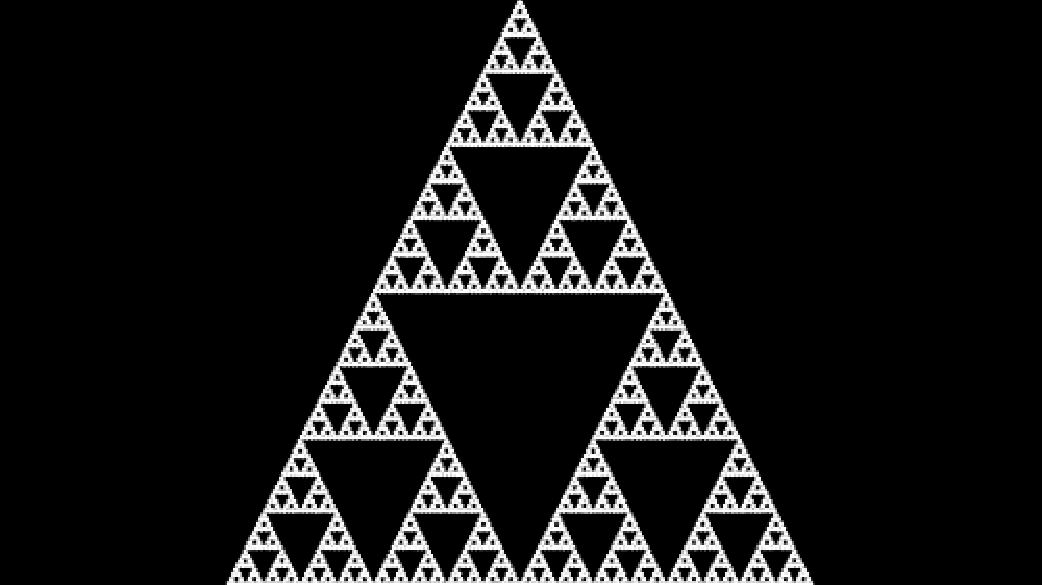
\includegraphics[width=3in, height=3in, keepaspectratio]{../img/fractal/gasket.pdf}
    \caption{Sierpinski gasket}
    \label{fig:gasket}
 \end{center}
\end{figure}

\subsection{About Rendering}

この節では,近年よく使われるシェーダを用いたレンダリング手法について触れる. 

最近のデモ作品でよく用いられる作品制作手法の1つに{\it OpenGL Shading Language(GLSL)}や{\it High Level Shading Language(HLSL)}の\emph{フラグメントシェーダ}(Fragment Shader)を用いるものがある.フラグメントシェーダは本来,ポリゴンに陰影をつけるために使用されるが,スクリーンスペースに矩形のポリゴンをレンダリングすることで各ピクセルごとの処理を記述しレンダリングすることができる.GPUは並列演算性能に優れていることに加え,各ピクセルの演算は並列に行われるため高速である. 

シェーダを用いたレンダリングでは, 全てのオブジェクトがプログラムで表現される.
例えば,  通常三次元物体を表現する場合には, メッシュで表現される. 
頂点や法線の情報を読み出して描画する.
それに対して, アルゴリズムで形状を生成することになる.  
小さなプログラムサイズでリアルタイムにレンダリングするという目的に合致する. 

例えば, フラグメントシェーダで円を描くことを考えてみる. 
原点中心,半径$r$の円の距離関数は以下のようになる.
\begin{eqnarray*}
 f(z) = | length(z) - r |
\end{eqnarray*}
この関数は円周からの距離を返す.この距離から一定以下の距離をもつ時にピクセルを塗りつぶす処理を書くと円を描くことができる.複数の図形を描きたい時は,複数の距離関数を評価し,最も小さな距離を求めればよい.
また,距離関数は陰関数とその微分から近似的に導出することができる.与えられた点$x$に対して, 陰関数$f(x)$が表す零点集合への最短距離を返す距離関数は以下のように近似的に求めることができる. 
\begin{eqnarray*}
 DistanceFunction(x) \approx \frac{|f(x)|}{|\bigtriangledown f(x)|}
\end{eqnarray*}
この手法はDistance Estimationと呼ばれ,複雑な形状を高速かつ綺麗に描画することに役立つ.この形は基本形であるが, より精度の高い近似式を得るための工夫が施される場合がある. 詳しい導出はInigo Quilez氏の記述が詳しい\footnote{distance estimation: \url{http://iquilezles.org/www/articles/distance/distance.htm}}.

シェーダで三次元空間を描画する場合には\emph{レイトレーシング}({\it Ray tracing})が用いられる.レイトレーシングは視点からスクリーンへ\emph{レイ}({\it Ray})を飛ばし,その挙動をシミュレーションすることで物体を描画する手法である.レイと物体の交差点はレイの方向と位置から代数的に計算することができる.
また,\emph{レイマーチング}({\it Ray marching, Sphere tracing}とも呼ばれる)\cite{sphereTracing}という手法を用いるこfとで,距離関数を用いて任意の三次元形状との交差点を近似的に計算することができる.物体の形状を代数的に計算することが難しいフラクタル形状のレンダリングを行う際は,Distance Estimationにより近似的に物体との距離を得てレイマーチングを用いることで,高速に描画することができる.

GLSLによるレンダリングや,レイマーチングに関しては,doxas氏のwgld\footnote{wgld: \url{https://wgld.org/d/glsl/}}によくまとまっている.シェーダを用いたレンダリングはglslsandbox\footnote{glslsandbox: \url{http://glslsandbox.com/}}やShadertoy\footnote{Shadertoy: \url{https://www.shadertoy.com/}}といったウェブサービスで手軽に試すことができる.

GPUの計算性能をより汎用的な計算に用いるためのプラットフォームとしてCUDAやOpenCLが登場している.これらのプラットフォームを用いることでシェーダではできない複雑な処理を行うことができるようになり,GPUは機械学習などの分野にも活躍の場を広げた.このようにGPUによる演算を画像処理以外の汎用的な用途に用いる技術はGPGPUと呼ばれている.

\subsection{Escape-time Fractals}
{\it Escape-time Fractals}は複素平面上の点に対して,特定の漸化式を計算し,その点の軌道の収束,発散を見ることで描画されるフラクタルである.
Escape-time Fractalsで代表的なものが\emph{マンデルブロ集合}({\it Mandelbrot set})である. 
マンデルブロ集合の漸化式は以下のようになる.
\begin{eqnarray*}
 \begin{cases}
  z_{n+1} = z^2_{n} + c \\ z_0 = 0
 \end{cases}
\end{eqnarray*}
$z_n$が無限大に発散しないものをマンデルブロ集合と呼ぶ.図\ref{fig:mandelbrot}は黒い部分がマンデルブロ集合である.発散と判定されるまでの計算の回数によって色をつけた.
マンデルブロ集合はその単純な式から驚くほど豊富なバリエーションの図を見ることができる.
その他のEscape-time fractalには,\emph{ジュリア集合}({\it Julia set})(図\ref{fig:julia})や\emph{ファトゥー集合}({\it Fatou set})等がある.

各点における漸化式の計算はお互いに干渉しないので,そのままシェーダでの実装が可能であるが,先に述べたDistance Estimationを用いることで,エイリアシングノイズ等を避けてより精細に描画することができる.これには{\it Green Function}と呼ばれる陰関数を用いる.導出はiq氏の記事が詳しい\footnote{distance rendering for fractals: \url{http://iquilezles.org/www/articles/distancefractals/distancefractals.htm}}.Green Functionに関しては,マンデルブロ集合に関する詳細な議論となってしまうので,こちらの論文\cite{mandelbrot}を参考にされたい.

\begin{figure}[htbp]
 \begin{minipage}{0.49\hsize}
  \begin{center}
   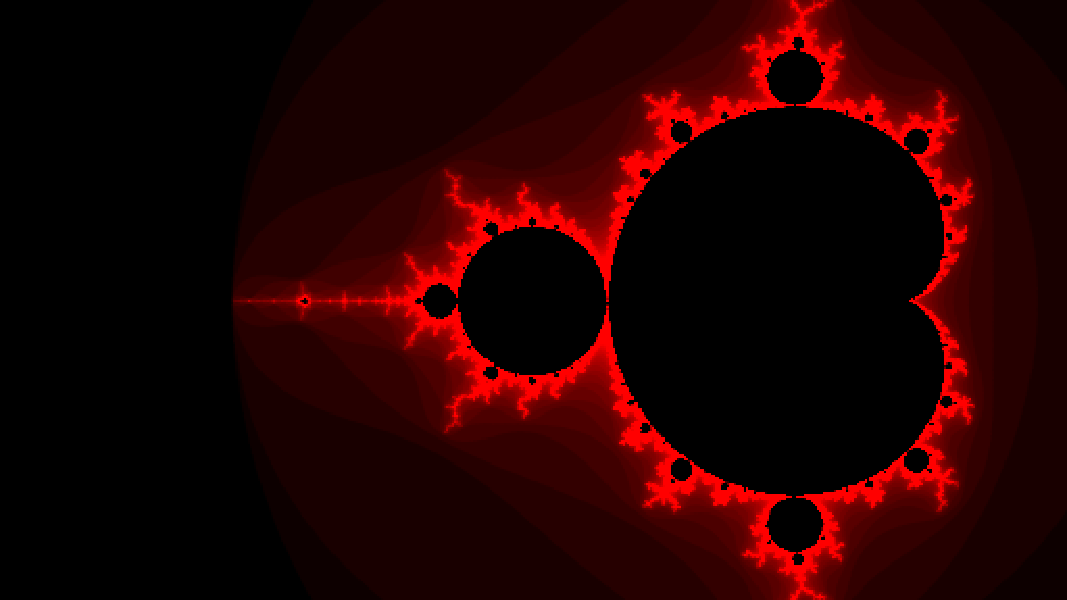
\includegraphics[width=3in, height=3in, keepaspectratio]{../img/fractal/mandelbrot.pdf}
   \caption{Mandelbrot set}
   \label{fig:mandelbrot}
  \end{center}
 \end{minipage}
 \begin{minipage}{0.49\hsize}
     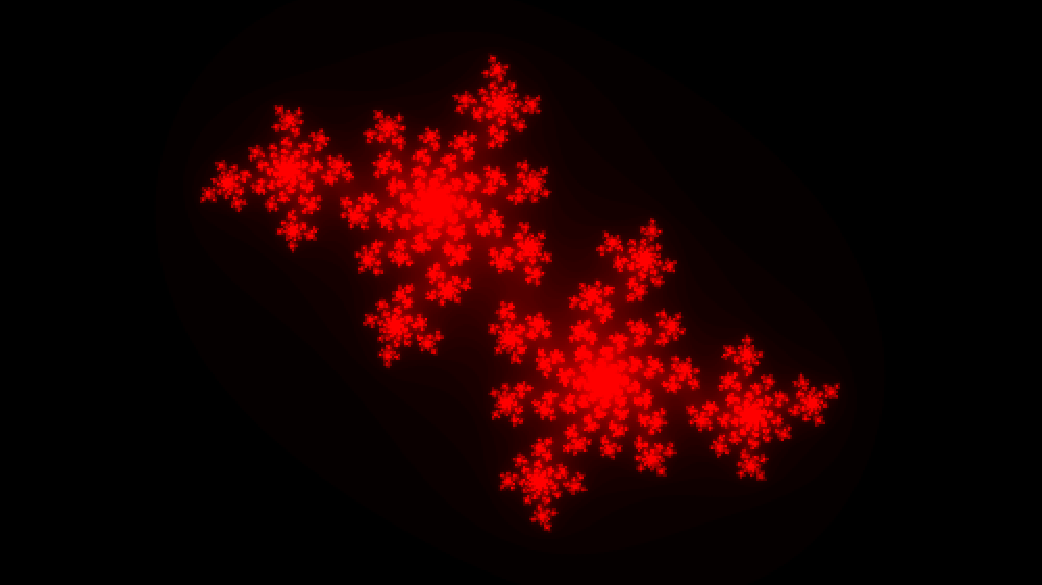
\includegraphics[width=3in, height=3in, keepaspectratio]{../img/fractal/julia.pdf}
   \caption{Julia set}
   \label{fig:julia}
 \end{minipage}
\end{figure}

\subsection{Distance Estimated 3D Fractals}

マンデルブロ集合のような複雑な3次元形状を持つフラクタルが求められていた.マンデルブロ集合を3次元に拡張する試みはさまざまに行われていたものの,あまり大きな成果はあげられていなかった.
例えば,ジュリア集合を4次元に拡張し,Distance Estimationを用いて描く方法が1989年には発表されている\cite{4djulia}.
しかし,その形状は単純でフラクタルコミュニティの満足のいくものではなかった.
2004年にKeenan Crane氏がGPUで実装した\footnote{Ray Tracing Quaternion Julia Sets on the GPU: \url{https://www.cs.cmu.edu/~kmcrane/Projects/QuaternionJulia/}}.

2003年に発表された阿原・荒木\cite{sphairahedra}による4次元クライン群の一種であるQuasi Fuchsian 3D Fractalsはある程度の複雑性を持った3次元フラクタルであり,コミュニティに大きな影響を与えたと言われている.このフラクタルに関しては後の章で触れる.その後,2009年にマンデルブロ集合をうまく三次元に拡張したMandelbulbの出現を皮切りに,次々と複雑な三次元フラクタルの式が発見された.これらもDistance Estimationとレイマーチングを用いることで効率よくレンダリングすることができる.これらのフラクタルはDistance Estimated 3D Fractalsと呼ばれることが多い.これらのフラクタルの歴史と実装についてはMikael Hvidtfeldt Christensen氏のSyntopiaの一連のブログポスト\footnote{Syntopia, Distance Estimated 3D Fractals: \url{http://blog.hvidtfeldts.net/index.php/2011/06/distance-estimated-3d-fractals-part-i/}}によくまとめられている.

これらフラクタルをレンダリングするためのソフトウェアはMandelbulb 3D\footnote{Mandelbulb 3D: \url{http://mandelbulb.com/2014/mandelbulb-3d-mb3d-fractal-rendering-software/}}やMandelbulber\footnote{Mandelbulber: \url{http://www.mandelbulber.com/}}が有名である.
Fragmentarium\footnote{Fragmentarium: \url{http://syntopia.github.io/Fragmentarium/}}はシェーダベースのグラフィクスを開発するための環境である.フラクタルのサンプルコードも豊富で学習に役立つ.
Fractal Lab\footnote{Fractal Lab: \url{http://hirnsohle.de/test/fractalLab/}}はブラウザ上でGLSLを用いてフラクタルをレンダリングすることができるWebアプリケーションである.この章で使われている図のいくつかはFractal Labを用いてレンダリングした.

\subsubsection{Mandelbulb}

マンデルブロ集合を三次元に拡張するにあたって一番の問題は漸化式の意味付けであった.
マンデルブロ集合では複素平面上で計算を行なうため, $z^2$は回転と拡縮, $c$の加算は点の平行移動を表わし, それによって軌道を見ることができる. 
三次元空間の点において, 同様の意味を表わす代数体系のようなものを考える必要があった. 
様々なアプローチが考案されたが, 最終的にD.White(twinbee)氏とP.Nylander氏が開発したMandelbulbが広く知られるようになった. 

White氏は球面座標上で漸化式を計算するアプローチを提案\footnote{\url{http://www.fractalforums.com/3d-fractal-generation/true-3d-mandlebrot-type-fractal/}}した.
図\ref{fig:mandelbulb2}は$z_{n+1} = z_n^2 + c$を用いてレンダリングした結果であるが,あまり複雑な形状は現れなかった.
しかし,その後Nylander氏が式を高次の積を扱えるように拡張した.
図\ref{fig:mandelbulb8}は$z_{n+1} = z_n^8 + c $という式でレンダリングされた形状であり,Mandelbulbとして広く知られている.White氏のWebページ\footnote{Skytopia: \url{http://www.skytopia.com/project/fractal/mandelbulb.html}}では開発の詳しい経緯がまとめられている.

Mandelbulbは三次元空間の点に対して漸化式を計算することで形状を得ることもできるが, 通常はマンデルブロ集合と同様に距離関数を導出し, レイマーチングを用いてレンダリングする.

\begin{figure}[h!tbp]
 \begin{subfigure}{0.49\hsize}
   \begin{center}
    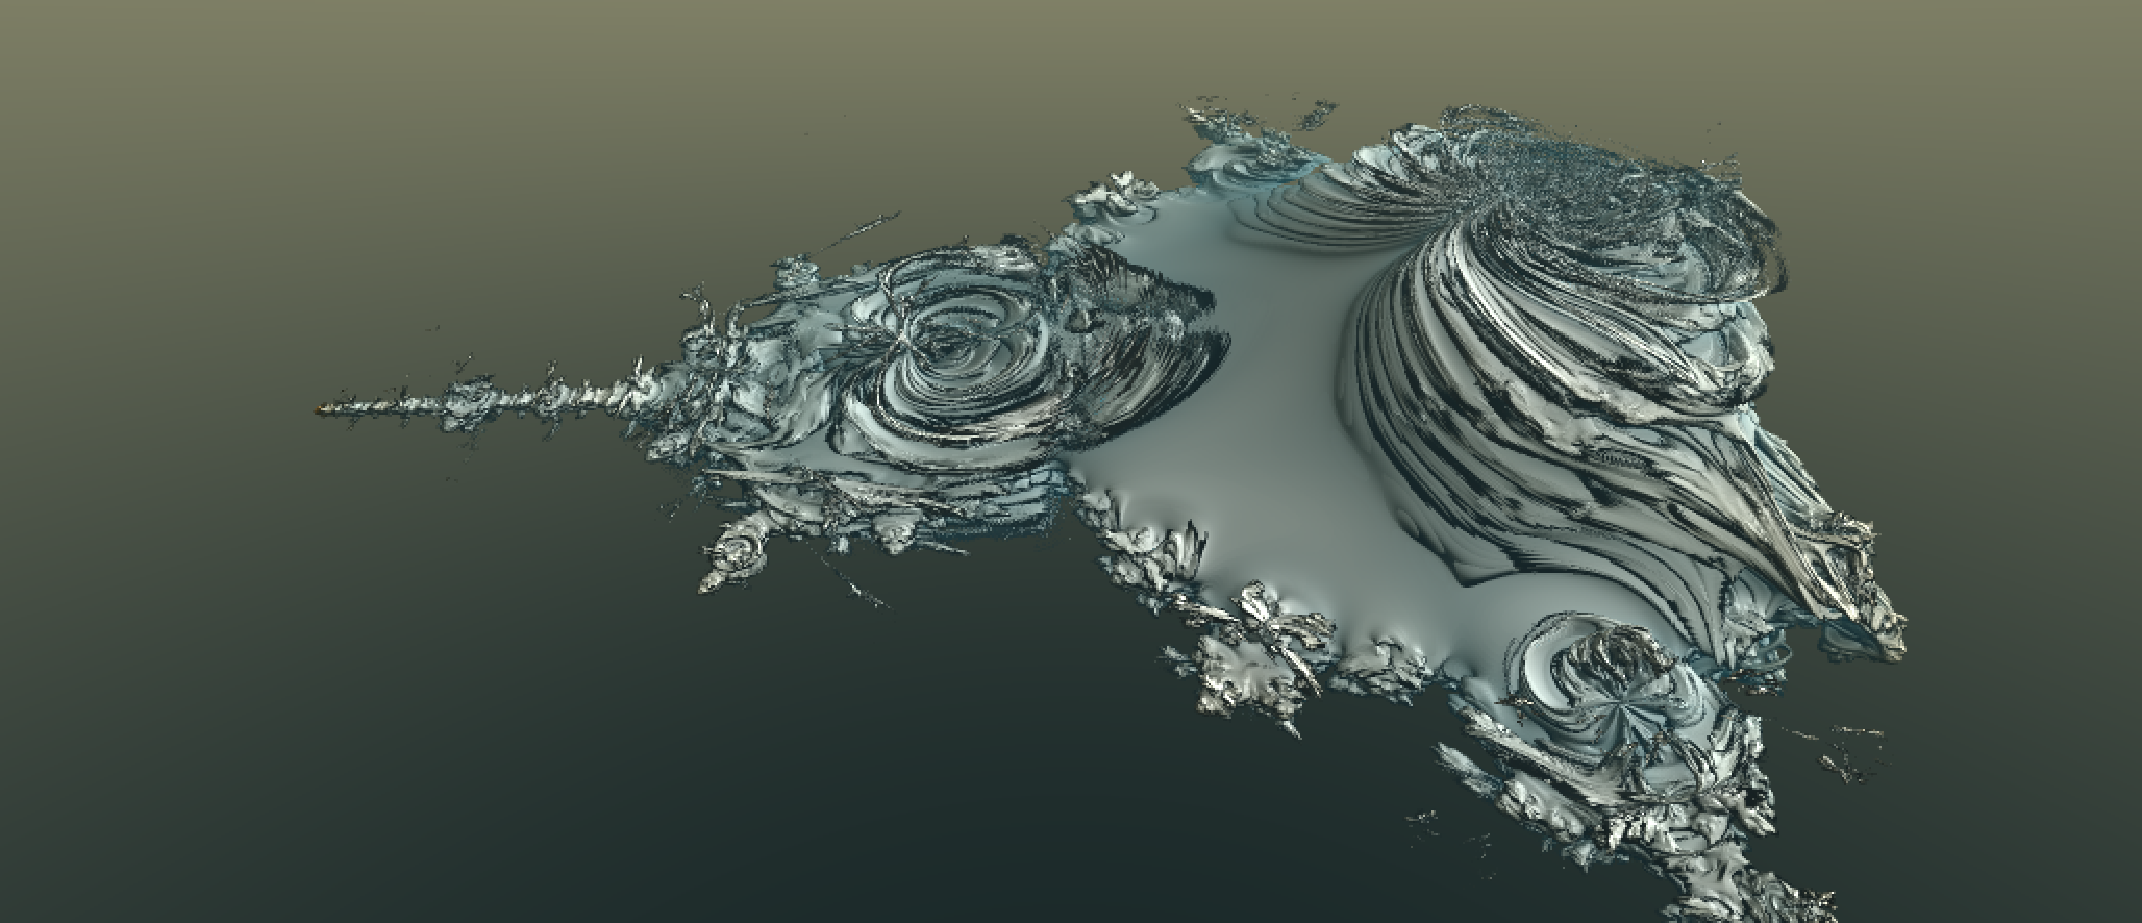
\includegraphics[width=3in, height=3in, keepaspectratio]{../img/fractal/mandelbulb2.pdf}
    \caption{$z_{n + 1} = z_n^2 + c$}
    \label{fig:mandelbulb2}
   \end{center}
 \end{subfigure}
 \hspace*{\fill}
 \begin{subfigure}{0.49\hsize}
   \begin{center}
    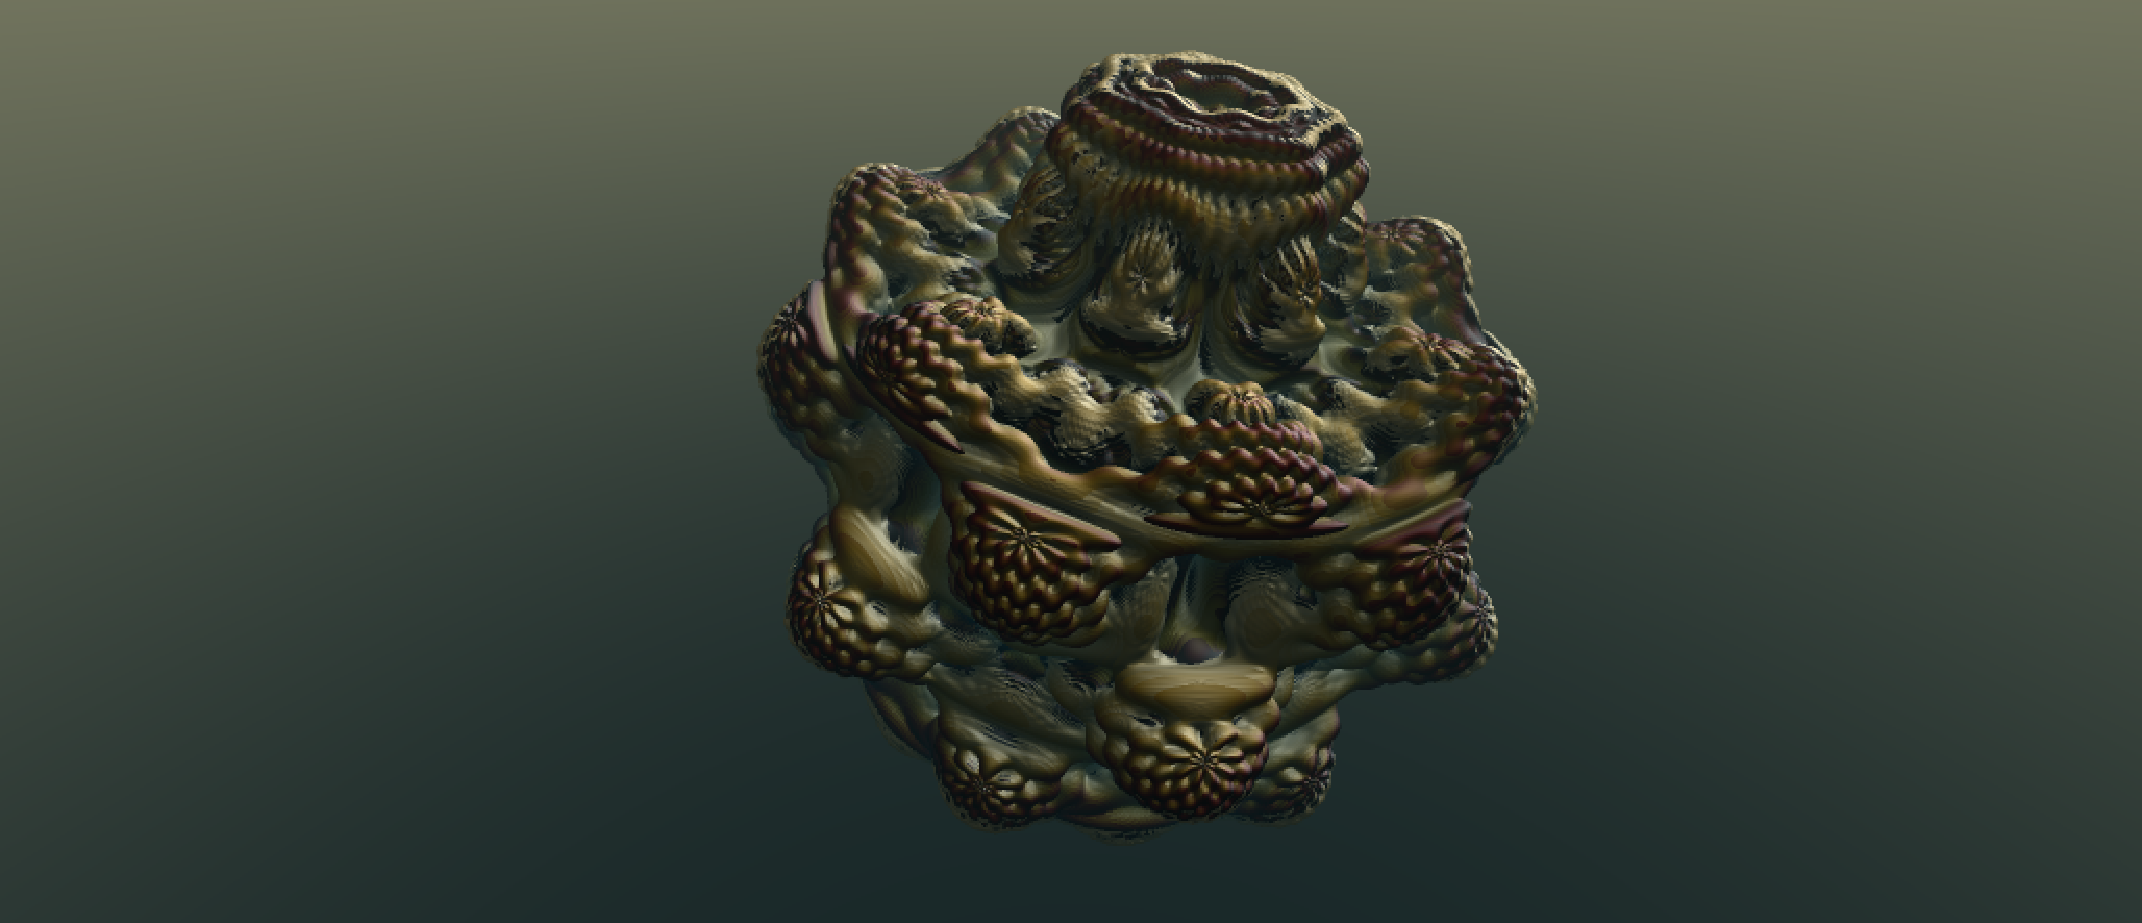
\includegraphics[width=3in, height=3in, keepaspectratio]{../img/fractal/mandelbulb8.pdf}
    \caption{$z_{n+1} = z_n^8 + c$}
    \label{fig:mandelbulb8}
   \end{center}
 \end{subfigure}
 \caption{Mandelbulb rendered by Fractal Lab}
\end{figure}

\subsubsection{Mandelbox}
その後,2010年にTom Lowe氏によってMandelbox\footnote{Mandelbox, \url{https://sites.google.com/site/mandelbox/what-is-a-mandelbox}}が開発された.
Mandelboxも三次元空間におけるEscape-time fractalである. 
漸化式は$z_{n+1} = scale * spherefold(minR, boxfold(z_n)) + c$となる.
ここで, boxfoldは$x=\pm1, y=\pm1, z=\pm1$を頂点にもつ立方体の各面に対して, 点が外側にある場合にその面に関する反転を行なう操作である.
また, spherefoldは以下の式で定義される.
\begin{eqnarray*}
 spherefold(r, z) = \begin{cases}
                  \frac{z}{r^2} & 0 \le |z| < r \\
                  \frac{z}{|z|^2} & r \le |z|
                 \end{cases}
\end{eqnarray*}
基本は原点中心, 半径1の球に関する反転である. 
球の反転は, 中心を無限遠点へ変換するが, Escape-timeアルゴリズムでは中心付近のほとんどの点が発散と判定されてしまう. 
そこでspherefoldでは, 中心付近の点の反転をあらかじめ決めておいた最小の半径における反転で制限をかけている.

Distance Estimationでは漸化式の微分としてヤコビアンの積を用いる. 
式の各操作のたびに, ヤコビアンを累積していき, 
最終的な点のノルムをヤコビアンの積で割ることで距離を近似的に求めることができる.

\begin{figure}[h!tbp]
 \begin{subfigure}{0.49\hsize}
   \begin{center}
    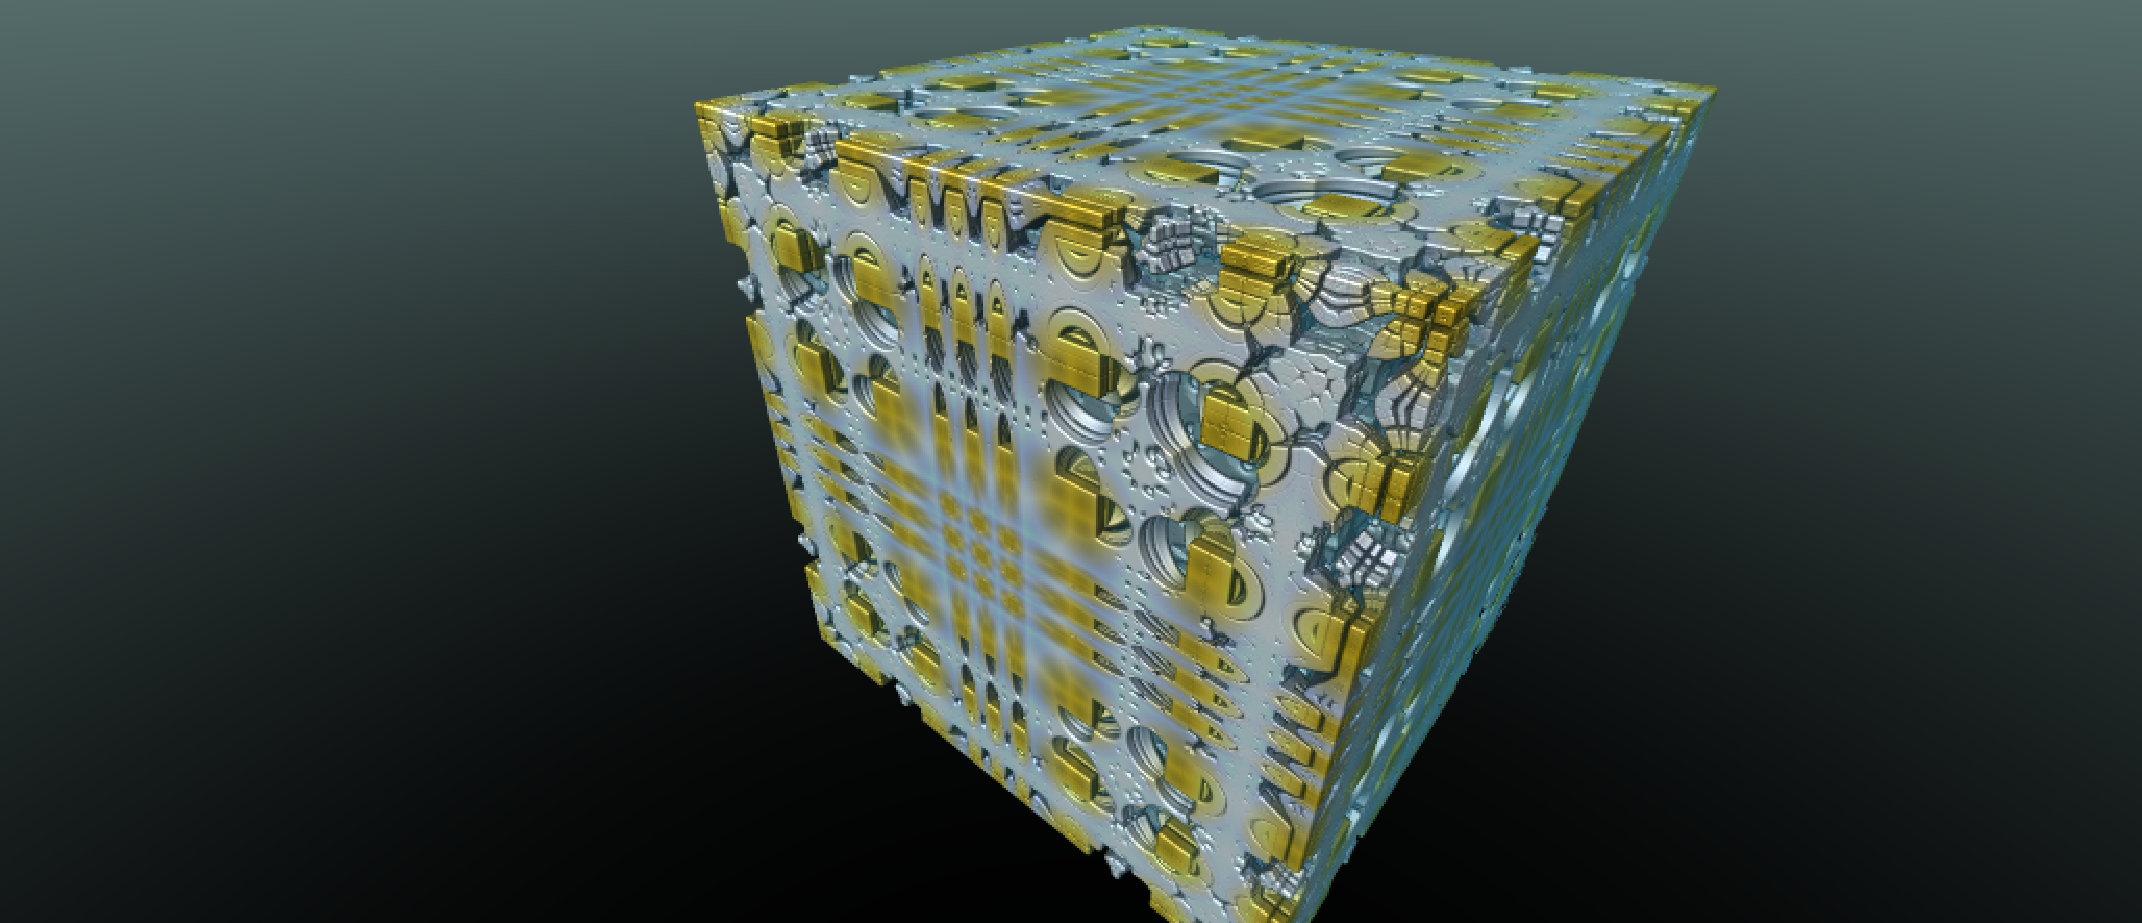
\includegraphics[width=3in, height=3in, keepaspectratio]{../img/fractal/mandelbox.pdf}
    \caption{}
    \label{fig:mandelbox1}
   \end{center}
 \end{subfigure}
 \hspace*{\fill}
 \begin{subfigure}{0.49\hsize}
   \begin{center}
    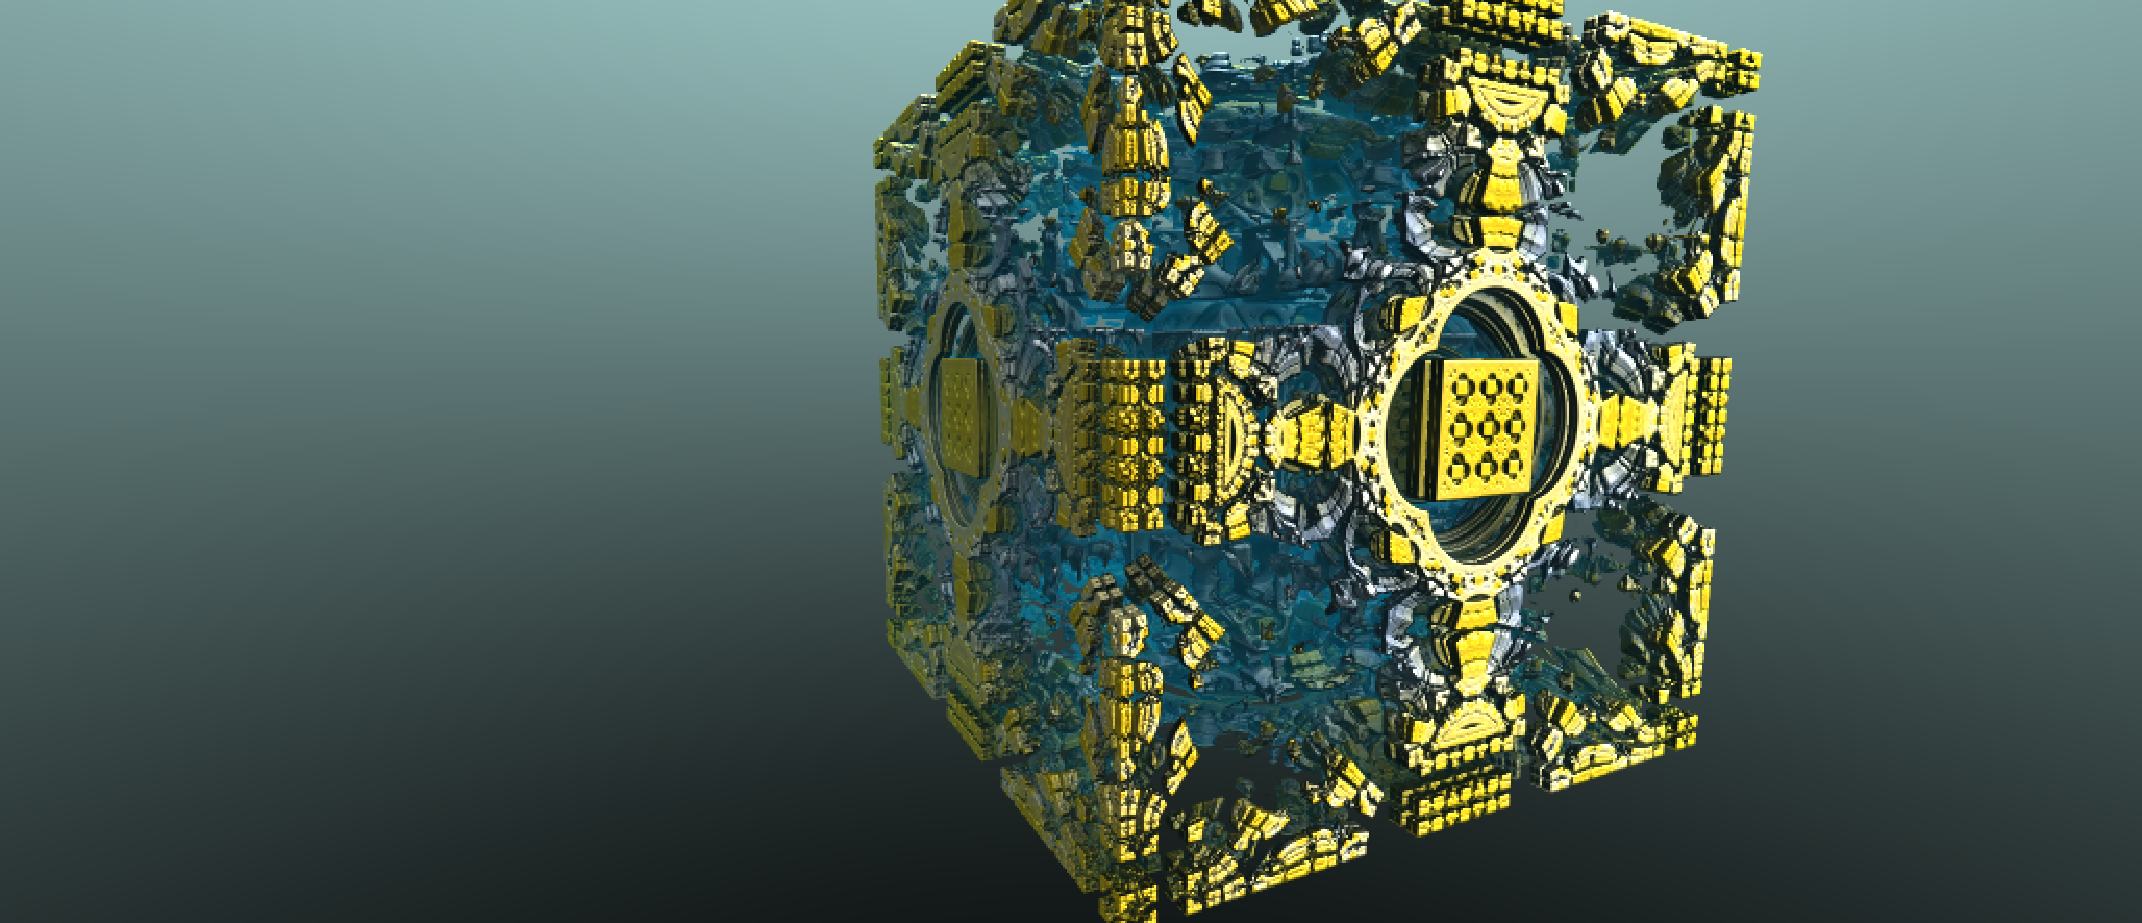
\includegraphics[width=3in, height=3in, keepaspectratio]{../img/fractal/mandelbox2.pdf}
    \caption{}
    \label{fig:mandelbox2}
   \end{center}
 \end{subfigure}
 \caption{Mandelbox rendered by Fractal Lab}
 \label{fig:mandelbox}
\end{figure}


\subsubsection{Pseudo-Kleinian}

Mandelboxの登場以降は漸化式にMandelbulbやMandelboxを含む複数の式を用いた{\it Hybrid System}によって.今も様々なフラクタル作品が作られている.
興味深いHybrid Systemの1つに{\it pseudo-kleinian}がある.これは球の反転に近い操作であるSpherefoldと平行移動と同じような働きをするboxfoldの組み合わせによってクライン群のような形状が得られる式である.図はfragmentariumのサンプルスクリプトを用いてレンダリングされた.

\subsection{Coloring by Orbit Trap}

Escape-timeアルゴリズムを用いたフラクタルのレンダリングでは,主に{\it Orbit Trap}というカラーリングの手法が使われる.trapと呼ばれる点や直線などの図形を空間上に置いておき,trapと軌道上の点の位置関係から色を付ける.図\ref{fig:mandelbox}のMandelboxもOrbit Trapを用いて色が着けられている.
図\ref{fig:mandelbrotOrbit}はマンデルブロ集合の計算によって$z_n$が桃色の領域に入った点を白く塗った.
桃色の領域に到達するまでの軌道を描いたといえる. この方法を応用すると,図\ref{fig:mandelbrotBitmap}のように画像をtrapに用いることで,点の軌道上に画像を張り付けることも可能である.この手法は特に{\it Bitmap Orbit Trap}とも呼ばれる.

\begin{figure}[htbp]
 \begin{minipage}{0.49\hsize}
  \begin{center}
   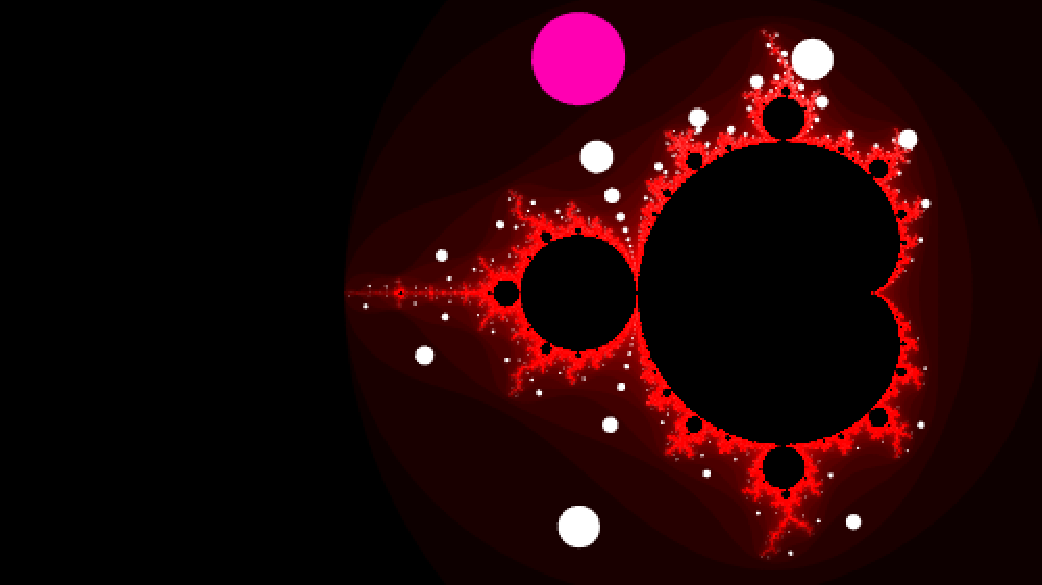
\includegraphics[width=3in, height=3in, keepaspectratio]{../img/fractal/mandelbrot-orbit.pdf}
    \caption{Mandelbrot set}
    \label{fig:mandelbrotOrbit}
  \end{center}
 \end{minipage}
 \begin{minipage}{0.49\hsize}
  \begin{center}
   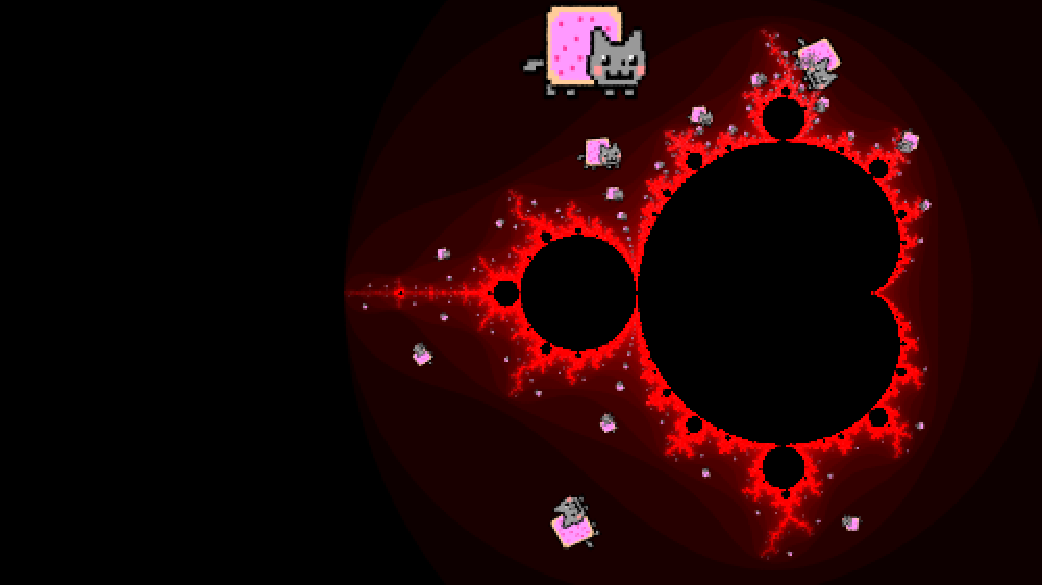
\includegraphics[width=3in, height=3in, keepaspectratio]{../img/fractal/mandelbrot-bitmap.pdf}
   \caption{Mandelbrot set}
   \label{fig:mandelbrotBitmap}
  \end{center}
 \end{minipage}
\end{figure}

\subsection{Other Fractals}

Iterated Function system(IFS)は点に様々な関数を適用して,その集積点をレンダリングするアルゴリズムである.シェルピンスキーのギャスケットなどもIFSでレンダリングすることができる.
IFSに関する書籍としてはFractals Everywhere\cite{fractalsEverywhere}が有名である.並列計算による高速化に関して以下の論文にまとめられている\cite{highPerformanceIFS}\cite{GPUIFS}.
IFSの一種にフラクタルフレーム(Fractal Frame)\cite{fractalFrame}と呼ばれるものがある.フラクタルフレームはIFSに用いる関数にメビウス変換などの非線形変換を用い,美しくレンダリングされるようにカラーリングが工夫されている.

他にも様々なアルゴリズムが存在するが,今回は後述するクライン群のレンダリングには関連してこないので触れない.マンデルブロ自身の著作\cite{fractal}では種々のフラクタルについて網羅的にまとめられている.
